%% ------------------------------------------------------- %%
%% Rodin
%% ------------------------------------------------------- %%
\section{Event-B and the Rodin platform}
Event-B is a formal method for system modeling. Key features of Event-B are the use of set theory as a modeling notation, the use of refinement to represent systems at different abstraction levels and the use of mathematical proof to verify consistency between refinement levels.

The Rodin platform is an Eclipse\cite{ECLIPSE}-based IDE for Event-B that provides effective support for refinement and mathematical proof. The releases\cite{RODIN} of the Rodin platform as well as the source files\cite{SOURCES} are available from the SourceForge site. The tool documentation for users and developers is provided within the Event-B wiki\cite{WIKI}.

\subsection{Contributing to the Rodin Platform}
The Rodin platform is Open Source and is extendable with plug-ins and extension points.

\begin{figure}
\centering
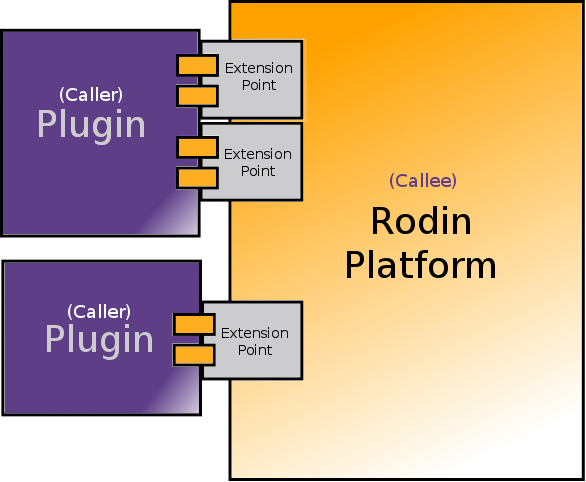
\includegraphics[scale=0.25]{Rodin.png}
\caption{Plug-ins and extension points} 
\label{Fig:Rodin Platform}
\end{figure}

In particular, it is possible to add new reasoners, which will schematically run as follows:
\begin{itemize}
\item Input: a sequent Hypotheses $\vdash$ Goal.
\item Invocation of an SMT solver.
\item Output: a proof rule.
\end{itemize}

\subsection{Integration of an SMT Solver into Rodin}
\begin{itemize}
\item A formula $A$ is \textit{valid} in a theory $T$ if $A$ evaluates to $true$ in every model $M$ of $T$.
\item A formula $A$ is \textit{satisfiable} in a theory $T$ if there is a model $M$ for $T$ in which $A$ evaluates to $true$. Otherwise, $A$ is \textit{unsatisfiable}.
\end{itemize}

It can be deduced that if a formula is unsatisfiable, its negation is valid. In other words, if $A \land \lnot B$ is unsatisfiable, then $A \limp B$ is valid. As a consequence, an Event-B sequent is not passed as is to an SMT solver, but its negation is taken as input by the SMT solver.
Conversely, if a formula is satisfiable, it means that a counter-example exists for its negation.

\begin{figure}
\centering
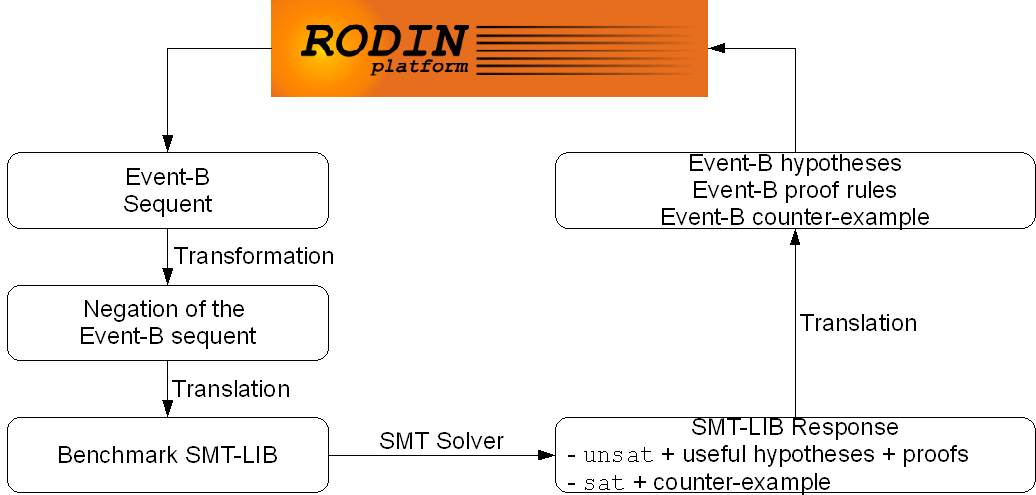
\includegraphics[scale=0.5]{Integration_SMT.png}
\caption{Integration of an SMT solver} 
\label{Fig:SMT solver}
\end{figure}

The main difficulties are all related to the translation steps. They cover several sub-tasks, such as selecting the hypotheses, choosing the SMT solver to be addressed, determining the format of the benchmark to be generated (SMT-LIB 1.2 or SMT-LIB 2.0), keeping a link between Event-B hypotheses and the associated hypotheses in SMT-LIB format...